\documentclass[aspectratio=169]{beamer}
\usepackage[brazil]{babel}
\usepackage[utf8]{inputenc}
\graphicspath{{Figuras/}}
\usepackage{graphics,amssymb,amsfonts,amsmath}
\usepackage{amsthm}
\usepackage{graphicx,subfig}
\usepackage{tabularx,arydshln}
\usepackage{booktabs,multirow,float,array}
\usepackage{enumerate,hyperref}
\usepackage{biblatex}
\usepackage{palatino}	
\usepackage{ragged2e}
\usepackage[utf8]{inputenc}
\setbeamertemplate{theorems}[numbered]
\usepackage{caption}

\addbibresource{refs.bib}

\usetheme{Berlin}
\usefonttheme[onlymath]{serif}
\setbeamertemplate{caption}[numbered]
\hypersetup{pdfpagemode=FullScreen}
\hypersetup{pdfpagelayout=SinglePage}

\newtheorem{teo}{Teorema}
\newtheorem{lema}[teo]{Lema}
\newtheorem{definicao}[teo]{Definição}
\newtheorem{exemplo}[teo]{Exemplo}
\newtheorem{exercicio}[teo]{}
\newtheorem{corolario}[teo]{Corolário}
\newtheorem{proposicao}[teo]{Proposição}
\newtheorem{observacao}[teo]{Observação}
\newenvironment{demonstracao}{\smallskip \noindent{\it Demonstração}: }
{\hfill $\Box$\hspace{1in}\medskip}

\logo{
\includegraphics[width=.15\textwidth]{Logo Ágora.jpeg}}

% Titulo: altere aqui seu título, autores e datas
\title[\sc{ÁGORA MATEMÁTICA 2025}]{Uma Generalização do Teorema do Valor Intermediário para Espaços Topológicos Arbitrários}
\author[Gasperi, João.; Prudencio, Jéssica]{João Paulo Chiari de Gasperi\\Jéssica Buzatto Prudencio}
\date[XX/09/2025]

\begin{document}
	
	
	\titlepage
	
	
	\AtBeginSubsection[]{
		\begin{frame}
			\frametitle{Sumário}
			\tableofcontents[currentsection, currentsubsection]
	\end{frame}}
	
	
	
	
	
	
	%%%%%%%%%%%%%%%%%%%%%%%%%%%%%%%%%%%%%%%%%%%%%%%%%%
	\section{Introdução}
	%os nomes das seções, subseções e blocos são sujestivos e podem ser alterados.
	
	\begin{frame}
		%blocos são opicionais
		\begin{block}{\centering{Teorema do Valor Intermediário}}
			Se $f:[a,b] \rightarrow \mathbb{R}$ é uma função contínua, onde $[a, b]$ é um intervalo real e $f(a) < f(b)$, então para todo $z \in (f(a), f(b))$ existe pelo menos um $c \in (a, b)$, onde $f(c) = z$
		\end{block}
		
		\begin{figure}[h!] 
			\centering 
			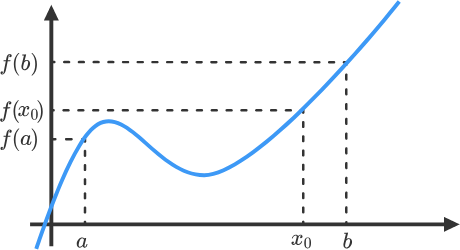
\includegraphics[width=0.4\textwidth]{tvi.png} % Passo 3: Incluir a imagem e ajustar a largura
			\caption{Teorema do valor intermediário.} 
			\label{fig:minha_imagem}
		\end{figure}
		
	\end{frame}
	
	\begin{frame}{Sumário}
		\tableofcontents
	\end{frame}
	
	
	%%%%%%%%%%%%%%%%%%%%%%%%%%%%%%
	\section{Desenvolvimento}
	
	%%%%%%%%%%%%%%%%%%%%%%%%%%%%%%%
	\subsection{Definições e propriedades Topológicas}
	%você pode adicionar mais subseções se quiser
	
	\begin{frame}{Definição de Topologia}
		Seja $X$ um conjunto qualquer. Uma Topologia sobre $X$ é um conjunto
		$\tau \subset \mathcal{P}(X) = \{A | A \subset X\}$ que satisfaz as seguintes propriedades:
		\begin{enumerate}
			\item $\emptyset, X \in \tau$;
			\item Uma união arbitrária de elementos de $\tau$ também está em $\tau$;
			\item Uma interseção finita de elementos de $\tau$ também está em $\tau$.
		\end{enumerate}
		
		%ok
		Se $U \in \tau$, dizemos que $U$ é aberto em $X$ sob a topologia $\tau$.
		Chamamos $(X, \tau)$ de espaço topológico.
	\end{frame}
	
	\begin{frame}{Exemplo}
		\begin{itemize}
			\item $\tau_1 = \mathcal{P}(X)$ - Topologia Discreta
			\item $\tau_2 = \{\emptyset, X\}$ - Topologia Indiscreta
		\end{itemize}
	\end{frame}
	
	\begin{frame}{Bases}
		Dizemos que $\mathcal{B}$ é uma base para uma topologia em $X$ se:
		\begin{enumerate}
			\item Para todo $x \in X$, existe $B \in \mathcal{B}$, onde $x \in B$;
			\item $B_1, B_2 \in \mathcal{B}$ e $x \in B_1 \cap B_2$, então existe $B \in \mathcal{B}$, tal que $x \in B \subset B_1 \cap B_2$.
		\end{enumerate}
		
		\begin{proposicao}
			Seja $\tau$ topologia gerada por uma base $\mathcal{B}$. Então $\tau$ é igual ao conjunto de todas as possíveis uniões dos elementos de $\mathcal{B}$.
		\end{proposicao}
	\end{frame}
	
	\begin{frame}{Topologia da Ordem}
		Seja $X$ um conjunto munido com uma relação de ordem linear.
		
		Definimos em $X$, a topologia gerada $\tau$ tomando como base os conjuntos: $(a, b), [a_0, b), (b, b_0], [a_0, b_0]$, onde $a, b \in X$ arbitrários, $a_0 = minX$ e $b_0 = maxX$, caso existam.
	\end{frame}
	
	\begin{frame}{Exemplo}
		Considerando $\mathbb{R}$ e a relação de ordem usual, a topologia da ordem é a que denonimamos por topologia canônica do conjunto $\mathbb{R}$.
		
		Os intervalos abertos da reta real são base para essa topologia.
	\end{frame}
	
	\begin{frame}{Topologia do Subespaço}
		Sejam $(X, \tau)$ um espaço topológico e $Y \subset X$. Definimos a topologia $\tau' = \{A \subset Y : A = U \cap Y, U \in \tau\}$ sobre $Y$ como a topologia do subespaço. 
		
		\begin{block}{Equivalentemente:}
			Os abertos em $Y$ são as interseções dos abertos de $X$ com $Y$.
		\end{block}
	\end{frame}
	
	\begin{frame}{Definições}
		\begin{minipage}{0.65\textwidth}
			Sejam $X$ um espaço topológico e $A \subset X$. Definimos:
			\begin{itemize}
				\item O interior de $A$, denotado por $intA$, como a união de todos os abertos de $X$ contidos em $A$.
				\item O fecho de $A$, denotado por $\bar{A}$, como a interseção de todos os fechados de $X$ que contém $A$;
				\item A fronteira de $A$, denotada por $\partial A$, que é o conjunto $\bar{A} - intA$.
			\end{itemize}
		\end{minipage}\hfill
		\begin{minipage}{0.3\textwidth}
			\centering
			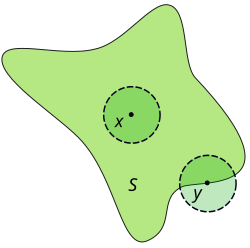
\includegraphics[width=\textwidth]{sets.png}
			\captionof{figure}{Interior, fecho e fronteira.}
			\label{fig:minha_imagem_2}
		\end{minipage}
	\end{frame}
	
	\subsection{Continuidade}
	
	\begin{frame}{Definição}
		Sejam $X, Y$ dois espaços topológicos e $f: X \to Y$ uma função. Dizemos que $f$ é contínua quando para todo conjunto $V$ aberto em $Y$, $f^{-1}(V)$ é aberto em $X$. 
	\end{frame}
	
	\begin{frame}{Exemplo}
		Sejam $X$ um espaço topológico e $A$ um conjunto discreto de $X$. Toda função $f$ definida em $A$ é contínua.
		
		Pois:
		\begin{itemize}
			\item Seja $V$ um aberto contido no contra-domínio de $f$;
			\item $f^{-1}(V) \subset A$, logo é aberto.
		\end{itemize}
		Caso particular: considerando $\mathbb{N} \subset \mathbb{R}$, nota-se que $f: \mathbb{N} \to \mathbb{R}$ é contínua.
	\end{frame}
	
	\begin{frame}{Homeomorfismo}
		Sejam $X, Y$ dois espaços topológicos. Se existe $f:X \to Y$ contínua, bijetora, com inversa contínua, então $f$ é chamada de homeomorfismo e os espaços $X$ e $Y$ são ditos homeomorfos.
	\end{frame}
	
	\subsection{Conexidade}
	
	\begin{frame}{Cisão}
		Uma cisão de $X$ é um par de conjuntos $A, B \subset X$, onde $A \cap B = \emptyset$, $A \cup B = X$ e $A, B$ são abertos em $X$.
	\end{frame}
	
	\begin{frame}{Conexidade}
		Dizemos que um conjunto é conexo quando a sua única cisão é a trivial.
	\end{frame}
	
	\begin{frame}{Continuidade e Conexidade}
		\begin{teo}
			A imagem de um conjunto conexo por uma função contínua é conexa.
		\end{teo}
	\end{frame}
	
	\begin{frame}{Teorema da Alfândega}
		\begin{teo}
			Seja $A \subset X$ um subespaço. Se $C \subset X$ é conexo e intercepta $A$ e o complemento de $A$, então $C$ também intercepta a fronteira de $A$.
		\end{teo}
	\end{frame}
	
	\subsection{Teorema do Valor Intermediário}
	
	\begin{frame}{Definições}
		Seja $X$ um conjunto munido com uma relação de ordem linear.
		\begin{itemize}
			\item $Y \subset X$ é convexo se, para todo $x, y \in X$, o conjunto $[x, y] = \{t \in X| x \le t \le y\}$ está contido em $Y$.
			\item $X$ é um contínuo linear se todo subconjunto limitado superiormente de $X$ tem supremo e para todo $x, y \in X$, existe um $z\in X$, onde $x < z < y$.
		\end{itemize}
	\end{frame}
	
	\begin{frame}{Intervalos}
		\begin{itemize}
			\item Seja $X$ um contínuo linear. Considerando a topologia da ordem, $Y \subset X$ é convexo se, e somente se, for um intervalo ou um raio.
			\item Seja $X$ um espaço topológico na topologia da ordem. $Y \subset X$ é conexo se, e somente se, é convexo.
		\end{itemize}
	\end{frame}
	
	\begin{frame}{TVI geral}
		Sejam $X, Y$ espaços topológicos e $f:X \to Y$ uma função, onde $X$ é conexo, $Y$ está munido com a topologia da ordem e $f$ é contínua. Se $a, b$ são dois pontos de $X$ tais que $f(a) < f(b)$ e $z \in Y$, onde $f(a) < z < f(b)$, então, existe $c \in X$, tal que $f(c) = z$.    
		
		Basta notar que:
		\begin{itemize}
			\item $f(X)$ é conexo, pois $f$ é contínua;
			\item $[f(a), f(b)] \subset f(X)$.
		\end{itemize}
	\end{frame}
	
	%%%%%%%%%%%%%%%%%
	\section{Conclusão}
	\begin{frame}{Conclusão}
		\begin{itemize}
			\item Definições e construções de topologia;
			\item Funções contínuas e suas propriedades;
			\item Conjuntos conexos e suas propriedades;
			\item Generalização do TVI como consequência das propriedades dos conjuntos conexos.
		\end{itemize}
	\end{frame}
	
	
	%%%%%%%%%%%%%%%%%%%%%%%%%%%%%%%%%%%%%%%%%%%%%%%%%%%%%%%%%%
	\section{Referências}
	
	%são apenas exemplos	
	\begin{frame}
		\begin{block}{Referências}
			\begin{thebibliography}{x}
			\footnotesize{
				
				\bibitem{ELON1} Lima, Elon L. {\bf Curso de Análise. Volume 1.} Rio de Janeiro: IMPA, 2019.
				
				\bibitem{ELON2} Lima, Elon L. {\bf Curso de Análise. Volume 2.} Rio de Janeiro: IMPA, 2020.
				
				\bibitem{Munkres} Munkres, James R. {\bf Topology.} Londres: Pearson, 2014.

				
			}
		\end{thebibliography}
		\end{block}
	\end{frame}

	
\end{document}